% Chapter 1

\chapter{Introducción} % Main chapter title

\label{Chapter1} % For referencing the chapter elsewhere, use \ref{Chapter1} 

%----------------------------------------------------------------------------------------

% Define some commands to keep the formatting separated from the content 
\newcommand{\keyword}[1]{\textbf{#1}}
\newcommand{\tabhead}[1]{\textbf{#1}}
\newcommand{\code}[1]{\texttt{#1}}
\newcommand{\file}[1]{\texttt{\bfseries#1}}
\newcommand{\option}[1]{\texttt{\itshape#1}}

%----------------------------------------------------------------------------------------
\section{Introducción}

El área de optimización multi-objetivo implica múltiples funciones objetivos que usualmente se encuentran en conflicto.
%
Los Algoritmos Evolutivos (EAs) se ajustan idealmente para resolver Problemas de Optimización Multi-objetivo (MOPs), ya que a diferencia de los enfoques teóricos, los Algoritmos Evolutivos Multi-objetivo (MOEAs) están diseñados para proporcionar varias soluciones bien distribuidas y próximas al frente de Pareto.
%
Una cualidad de los EAs, es su capacidad de proporcionar soluciones próximas a las regiones óptimas sin la necesidad de conocer la función objetivo, por lo tanto es usual su efectividad en problemas prácticos que pueden incluir la optimización de tiempos, costos, capacidades y otras características.
%


En sus inicios los MOEAs se desarrollaron principalmente bajo el concepto de dominancia, proporcionando soluciones próximas al frente de Pareto al considerar dos y tres funciones objetivo, sin embargo al incrementar el número de objetivos se ha demostrado que la presión de selección es afectada de forma exponencial ya que al aumentar el número de objetivos la cantidad de individuos no dominados crece significativamente.
%
Por otra parte también se desarrollaron MOEAs cuyo mecanismo de búsqueda está dirigido por los indicadores, principalmente los indicadores más utilizados de tipo \textit{Pareto compliance} incrementan su complejidad de forma exponencial conforme aumenta el número de objetivos, en resultado tienden a no ser factibles en MOPs de muchos objetivos.
%

En base a esto se desarrollaron técnicas alternativas donde se proporcionan vectores direccionales distribuídos en el simplex, estos vectores son implementados con un determinado enfoque, convirtiendo el problema multi-objetivo en varios problemas mono-objetivos, siendo de los más utilizados en problemas de muchos objetivos, sin embargo se ha observado que la geometría del frente de Pareto puede afectar la calidad de los resultados.


Se ha demostrado que el rendimiento de los EAs es afectado por la falta de soluciones diversas, que en el caso mono-objetivo es diagnosticado como convergencia prematura.
%
Por otra parte los MOEAs conservan un grado de diversidad implícito, ya que al mantener la soluciones bien distribuídas en el espacio objetivo, éstas tienden a mantener un grado de diversidad en el espacio de las variables de decisión.
%
No obtante, este grado de diversidad implícito puede no ser suficiente para proporcionar soluciones de calidad.

%--------------------------------------------------------
\section{Motivación}
La motivación principal de este trabajo es demostrar la importancia en considerar esquemas de diversidad en el área de optimización multi-objetivo.
%
Los temas de diversidad en los algoritmo evolutivos son de gran importancia ya que se ha demostrado su superioridad en problemas complejos y además ofrecen un buen grado de estabilidad.
%
Principalmente, los algoritmos basados en diversidad demuestran su superioridad en ejecuciones a largo plazo, en base a esto y al incremento de las capacidades tecnológicas se ha vuelto un tema de interés en el área de las metaheurísticas poblacionales.

\section{Descripción del problema}

Los MOEAs conservan un grado de diversidad de forma implícita, ya que mantienen soluciones diversas en el espacio objetivo, sin embargo existen escenarios en donde los individuos son ubicados en regiones suboptimas y por lo tanto se estanca el proceso de búsqueda, en consecuencia no son alcanzadas las regiones que corresponden a los óptimos globales.
%


%--------------------------------------------------------
%%\section{Hipótesis}
%%\begin{itemize}
%%\item Los algoritmos evolutivos actuales están basados en mantener una buena diversidad en el espacio objetivo.
%%\item Esta tesis parte de la hipótesis que esto no es suficiente para mantener una buena diversidad en el espacio de las variables y que por lo tanto puede haber una convergencia prematura y no ofrecer buenos resultados a largo plazo.
%%\end{itemize}

%--------------------------------------------------------

\section{Objtivo general}

Diseñar y analizar dos algoritmos multi-objetivo para administrar la diversidad explícitamente y de forma simultánea tanto en el espacio de las variables como en el espacio de los objetivos, esto por medio de un esquema de selección o fase de remplazo con el propósivo se ofrecer soluciones de calidad y estabilidad en ejecuciones a largo plazo.

\section{Objetivos específicos}

\begin{itemize}
\item Analizar la influencia que existe de la diversidad en el espacio de las variables en los algoritmos evolutivos muti-objetivo.
\item Diseñar e implementar dos algoritmos multi-objetivos para administrar la diversidad de forma explícita en esquemas de largo plazo, los dos algoritmos son basados en dominancia y descomposición respectivamente.
\item Analizar el efecto que tiene el operador de cruce SBX y los operadores de evolución diferencial en los esquemas de diversidad.
\end{itemize}

%--------------------------------------------------------
\section{Análisis preliminar}

En las últimas decadas, una gran cantidad de MOEAs han sido desarrollados con el obejtivo de obtener buenas aproximaciones al frente de Pareto.
%In the last decades, a large amount of MOEAs  have been devised with the aim of obtaining proper approximations of the Pareto fronts.
%
Se consideran dos metas: las soluciones deberían estar próximas al frente de Pareto, y su diversidad debe ser maximizada (\cite{Joel:TUTORIAL_EMOA}).
%Two aims are usually considered: the solutions should be close to the Pareto front, and the diversity of the approximation should be maximized~\cite{Joel:TUTORIAL_EMOA}.
%
El diseño de los MOEAs que pertenecen al estado-del-arte usualmente consideran los dos procesos previamente mencionados, por lo tanto la calidad y diversidad de las soluciones en el espacio objetivo es considerada de forma explícita.
%The design of state-of-the-art MOEAs usually considers both previously mentioned purposes, i.e. the quality and the diversity of the solutions in the objective space are explicitly considered.
En el caso de dominios mono-objetivo, únicamente existe una meta en el proceso de optimización.
%In the case of single-objective domain, there is only one purpose in the optimization process.
%
Sin embargo, se ha demostrado de forma experimental que al integrar las reglas para promover la diversidad en el espacio de las variables puede generar ciertos beneficios en la calidad de las soluciones aproximadas.
%However, it has been found experimentally that integrating rules to promote the diversity in the variable space can bring benefits in terms of the objective function.
%
La principal razón es que los EAs tienden a perder la diversidad rápidamente, por lo tanto se podría tener una convergencia prematura.
%The main reason behind this finding is that EAs have a tendency to quickly lose diversity, so premature convergence might appear, meaning that many resources might be wasted.
%
Recientemene, se ha utilizado de forma exitosa un nuevo principio para obtener mejores resultados que los conocidos en varios problemas mono-objetivo (\cite{Joel:MULTI_DYNAMIC}).
%Recently, a new principle of design have been successfully used to obtain new best-known solutions in several well-known single-objective problems~\cite{Joel:MULTI_DYNAMIC}.
%
La idea principal consiste en relacionar la cantidad de diversidad mantenida en el espacio de las variables con el crierio de paro, el cual es asignado por el usuario.
%The main idea is to relate the amount of diversity maintained in the variable space to the stopping criterion set by the user.
%
Así, en las fases iniciales se induce una mayor capacidad de exploración al mantener un grado elevado de diversidad, mientras que en las fases finales se promueve un nivel de explotación debido a que el grado de diversidad va decrementándose de forma paulatina.
%Particularly, in the initial phases more exploration is induced by maintaining a large diversity whereas in the final phases exploitation is promoted by allowing some loss of diversity.
%
El criterio de paro es utilizado para promover un cambio gradual entre estas fases.
%The stopping criterion is used to promote a gradual change between these stages.

En muchos MOEAs recientes no se logra una convegencia completa debido a que se mantiene un grado de diversidad explícitamente en el espacio de los objetivos.
%In most current MOEAs, complete convergence can not appear because some degree of diversity is explicitly maintained in the multi-objective space.
%
De hecho, en algunos problemas mono-objetivo donde la convergencia prematura es un problema, se ha implementado la multi-objetivización como una forma para incrementar la diversidad con la meta de obtener soluciones de alta calidad (\cite{Joel:MOEAS_CONSTRAINED}).
%In fact, in some single-objective problems where premature convergence is an issue, multiobjectivization has been used as a way of increasing the diversity with the expectation of attaining higher-quality solutions~\cite{Joel:MOEAS_CONSTRAINED}.
%
Sin embargo, nuestra hipótesis consiste en que dependiendo del problema, la cantidad total de diversidad mantenida en el espacio de las variables puede ser mínima.
%However, our hypothesis is that depending on the problem, the total amount of diversity maintained in the variable space might be too low.
%
Por lo tanto podría aparecer una situación similar a la convergencia prematura donde el grado de diversidad podría no ser suficiente para mejorar los resultados.
%In such cases, a situation similar to premature convergence might appear with MOPs, i.e. the diversity might be not enough to improve further the results.

Para estudiar el desempeño de los MOEAs se han propuesto varios problemas de prueba (\cite{Joel:WFG_REVIEW}).
%Several benchmarks to study the performance of MOEAs have been proposed.~\cite{Joel:WFG_REVIEW}.
%
Entre ellos, uno de los más utilizados son los problemas WFG \textit{The Walking Fish Group}.
%Among them, the Walking Fish Group (WFG)~\cite{Joel:WFG} benchmark is one of the most widely accepted ones.
%
La herramienta WFG es utilizada para construir problemas de pruena de forma flexible.
%Los problemas WFG es una herramienta flexible para construir problemas de prueba bien diseñados.
%WFG is a flexible toolkit for constructing well-designed test problems.
%
En el artículo original, se construyeron nueve problemas de prueba como ejemplo.
%In the original paper, a benchmark consisting of nine test instances were built as an example.
%
Sin embargo estos nueve problemas se han utilizado popularmente y por lo tanto son seleccionados para realizar nuestros estudios.
%These nine tests are now quite popular and have been the ones selected to perform our studies.
%
Los problemas WFG dividen a las variables de decisión en dos tipos de parámetros: los parámetros de distancia y los parámetros de posición.
%The WFG problems divide the decision variables in two kinds of parameters: the distance parameters and the position parameters. 
%
Un parámetro $x_i$ es considerado un parámetro de distancia cuando para todos los parámetros del vector $\boldsymbol{\vec{a}}$, modificando $x_i$ en $\boldsymbol{\vec{a}}$ resulta en un parámetro que domina a $\boldsymbol{\vec{a}}$, es equivalente a $\boldsymbol{\vec{a}}$, o es dominado por $\boldsymbol{\vec{a}}$.
%A parameter $x_i$ is a distance parameter when for all parameter vectors \textbf{a}, modifying $x_i$ in \textbf{a} results in a parameter vector that dominates \textbf{a}, is equivalent to \textbf{a}, or is dominated by \textbf{a}. 
%
Por otra parte, $x_i$ es un parámetro de posición, si modicando $x_i$ en $\boldsymbol{\vec{a}}$ siempre resulta en un vector que es incomparable o equivalente a $\boldsymbol{\vec{a}}$ \footnote{Para mayor información se puede consultar el capítulo \ref{Chapter2} de este trabajo.}.
%However, if $x_i$ is a position parameter, modifying $x_i$ in \textbf{a} always results in a vector that is incomparable or equivalent to \textbf{a}. 

Es bien sabido que los MOEAs más recientes fallan con algunas de las funciones WFG más complejas.
%Nowadays, it is known that most current MOEAs fail with some of the most complex WFG benchmark functions. 
%
En esta sección demostramos que una de las razones es que, el estado-del-arte de los MOEAs no mantinenen un grado de diversidad suficiente.
%In this section we show that one of the reasons is that, state-of-the-art MOEAs do not maintain a high enough diversity.
%
Específicamente, se demuestra que la convergencia prematura aparece en los parámetros de distancia, que por lo tanto el operador de cruce pierde su poder de exploración.
%Particularly, it is shown that premature convergence appears in the set of distance parameters, meaning that the crossover lose its exploratory strength.
%
De hecho en estos casos, la única forma de mejorar los resultados es através del operador de mutación.
%In fact in such cases, the only way to improve further the results is through the application of mutation. 


En orden para ilustrar la debilidad previamente mencionada, se ha seleccionado el problema de prueba WFG1.
%In order to illustrate the previously mentioned drawback, the WFG1 test has been selected.
%
Se seleccionó el problema WFG1 porque posee una definición simple, pero muchos MOEAs tienen dificultades en resolverlo.
%We selected WFG1 because it has a relatively simple definition, but most current MOEAs face difficulties with it.
%
Específicamente, la instancia WFG1 es un problema uni-modal y separable.
%In fact, WFG1 is a uni-modal and separable problem. 
%
La región óptima para la instancia WFG1 (\cite{Joel:WFG}) se muestra en la ecuación (\ref{OPTIMALSOLUTION}).
%The optimal solution for WFG1~\cite{Joel:WFG} is shown in (\ref{OPTIMALSOLUTION}).
%
En esta ecuación, $k$ es el número de parámetros de posición, y $n$ corresponde a la dimensionalidad.
%In this equation, $k$ is the number of position parameters, and n is the dimensionality.
%
Los parámetros de $k+1$ a $n$ son los parámetros de distancia.
%The parameters from $k + 1$ to $n$ are the distance parameters.
%
Esta ecuación muestra que las soluciones optimas de Pareto tiene exactamente los mismos valores en los parámetros de distancia.
%This equation shows that any Pareto optimal solution has exactly the same values in the distance parameters.
%
\begin{equation} \label{OPTIMALSOLUTION}
X_{i=k+1:n} =2i\ \times\ 0.35
\end{equation}



Para realizar las ejecuciones se utilizó el marco de trabajo conocido como \textit{jMetalcpp} (\cite{Joel:jMetal}).
%The jMetalcpp~\cite{Joel:jMetal} framework was used to perform our executions.
%
Tomando en cuenta el comportamiento estocástico de los MOEAs, se realizaron 35 ejecuciones independientes.
%Taking into account the stochastic behavior of MOEAs, 35 independent executions were run.
%
En todas las ejecuciones se asignó un criterio de paro a $50,000$ generaciones y se asignó el tamaño de problación a $250$.
%In all of them, the stopping criterion was set to $50,000$ generations and the size of the population was fixed to $250$. 
%
En orden para analizar la diversidad, se calculó la distancia Euclídea promedio entre los individuos (ADI), es decir, el valor promedio de entre todos los pares de individuos de la población.
%In order to analyze the diversity, the average Euclidean distance among individuals (ADI) is calculated, i.e. the mean value of all pairwise distances among individuals in the population is reported.

En la figura \ref{fig:Average_StateArtDiversityDistanceParameters} se muestra la evolución de la diversidad para los algoritmos GDE3, SMS-EMOA, MOEA/D y NSGA-II.
%Fig.~\ref{fig:Average_StateArtDiversityDistanceParameters} shows the evolution of the diversity for GDE3, SMS-EMOA, MOEA/D and NSGA-II.
%
En la parte superior izquierda se muestra la evolución de la diversidad cuando se toman en consideración todos los parámetros, mientras que en la parte superior derecha, únicamente se toman en cuenta a los parámetros de distancia.
%The left part shows the evolution of the diversity when taking into account the whole set of parameters, whereas in the right part, only the distance parameters are taken into account.
%
Es importante aclarar que se utiliza la escala logarítmica.
%
En el caso de los parámetros de distancia, las regiones donde no se muestra información, corresponde a las generaciones donde la distancia promedio es cero.
%Note that a logarithmic scale is used; in the case of the distance parameters, the regions where no information is plotted correspond to generations where the distance is 0.
%
Como se puede apreciar, todos los métodos mantienen un grado de diversidad cuando se consideran a todos los parámetros.
%As we can appreciate, all the methods maintain some degree of diversity when all the parameters are considered.
%
Sin embargo, cuando únicamente son considerados los parámetros de distancia, todos los métodos llegan a una distancia promedio de cero de forma rápida.
%
De hecho, aproximadamente después de $5,000$ generaciones todos los parámetros de distancia tienen una distancia promedio de cero.
%However, when the distance parameters are the only one considered, all the methods reach a zero distance quite fast. In fact, after about $5,000$ generations all of them have reached a generation where the distance is equal to zero.
%
Esto significa que relativamente en pocas generaciones, todos los métodos han convergido en los parámetros de distancia.
%This means that in relatively few generations, all the methods have converged in the distance parameters.
%
Se puede observar que la diversidad es recuperada en algunas generaciones, esto se debe al operador de mutación.
%We can see that in some generations, some degree of diversity is recovered; this is because of the action of the mutation.
%
En las superficies de cubrimiento logradas (Figura \ref{fig:Superficie_WFG1}) se puede observar que cada uno de los MOEAs seleccionados, cuya distancia es mantenida durante más generaciones están más cercanas al frente de Pareto.
%In the experimental validation section, the attainment surfaces show that, in every of these state-of-the-art MOEAs, the distance among the found solutions and the optimal solutions are not low.
%
Sin embargo, no se obtiene una convergencia completa al frente de Pareto.
%Entonces, no se resuelve este problema de pruena por la convergencia prematura en los parámetros de distancia.
%Thus, the solving of this test is failing because of premature convergence in the distance parameters.
%
De hecho, después de que se pierde la diversidad en los parámetros de distancia, los MOEAs básicamente están modificando sólo los parámeros de posición, por lo que en la mayoría del tiempo se está mejorando la diversidad en el espacio objetivo en lugar de la calidad en las soluciones.
%In fact, after this loss of diversity, the MOEAs are basically modifying the position parameters, so the majority of the time is invested in improving further the diversity instead of the quality.
Por lo tanto las soluciones permanecen en las mismas regiones del espacio factible y los parámetros de posición únicamente están cambian en dichas regiones a lo largo de la ejecución.
%

%The algorithms lost diversity on distance parameters, then stay in the same sub-space regions, by other way positions parameters  are still moving along execution, this provide well spread in Pareto front. The differential evolution algorithms (DE) have properties of intensification as


%We implement two metrics for compute diversity DCN and average distance, the first one is the Distance of Closest Neighbor (DCN) from equation (\ref{DCN}) as indicate~\cite{Joel:DCN} where $d_{i,j}$ is the Euclidean distance $ d_{i,j} =  \sqrt{ \sum_{k=1}^{Dim} (x_{i,k} - x_{j,k})^2}$ and $j$ is the closest individual in decision space from individual $i$  with population size $N$.
%%\begin{equation}\label{DCN}
%%DCN = \frac{1}{N} \sum_{i=1}^{N} d_{i,j} 
%%\end{equation}


%The evolution of the diversity is showed with DCN and average distance metrics which are implemented with a logarithmic scale.
%The DCN metric has a disadvantage, this occur when a group of individuals are closest and one individual is located a way from rest, this scenario affect DCN metric resulting a low DCN value.\\
%The left plot of the figure () show that the original MOEAD is the first one that lost diversity considering all parameters with DCN metric, algorithm GDE3 maintain the best diversity this can be misleading because a multi-objective problem demand a minimum of diversity for obtain a well spread solutions on Pareto front which is defined by position parameters, then is necessary inspect distance and position parameters separately\footnote{We refer the positions and distance parameters as sub-spaces.}. As we show the right plot of the figure(\ref{fig:DCN_StateArtDiversityDistanceParameters}) the SMS-EMOA loses the diversity with distance parameters and MOEA/D is the best preserving diversity until the generation 15000, the algorithms NSGA-II and MOEA/D have picks which are caused for the mutation operator since average distance is zero showed in figure (\ref{fig:Average_StateArtDiversityDistanceParameters}). The GDE3 maintain best diversity considering all parameters and sub-space of distance parameters.
%The algorithms lost diversity on distance parameters, then stay in the same sub-space regions, by other way positions parameters  are still moving along execution, this provide well spread in Pareto front. The differential evolution algorithms (DE) have properties of intensification as explain~\cite{Joel:OperatorAHX}, this is showed when GDE3 lost diversity can not generate picks inside on the figures (\ref{fig:DCN_StateArtDiversityDistanceParameters}) and (\ref{fig:Average_StateArtDiversityDistanceParameters}), the reason is that mutation operator is missing, then GDE3 locate individuals inside of regions with non-dominated individuals and diversity on distance parameter is lost. The position parameter are still moving causing high diversity metrics, even more affecting metric diversity in all parameters.
\begin{figure}[H]
\centering
\begin{tabular}{cc}
    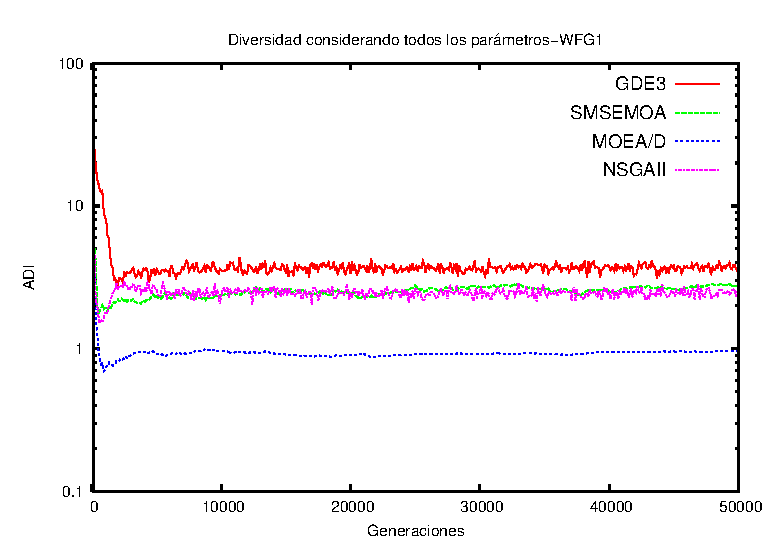
\includegraphics[width=0.5\textwidth]{Figures_Chapter1/Average_FullParamsStateArt.eps} 
    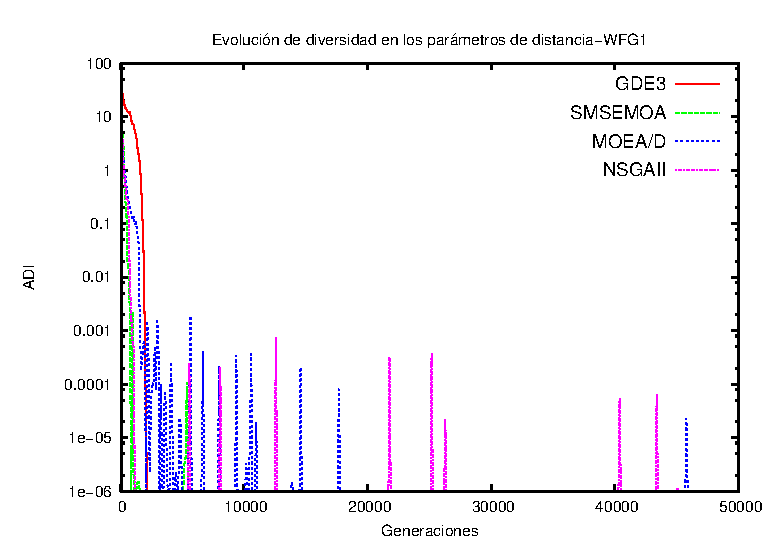
\includegraphics[width=0.5\textwidth]{Figures_Chapter1/Average_DistanceParamsStateArt.eps}  \\
    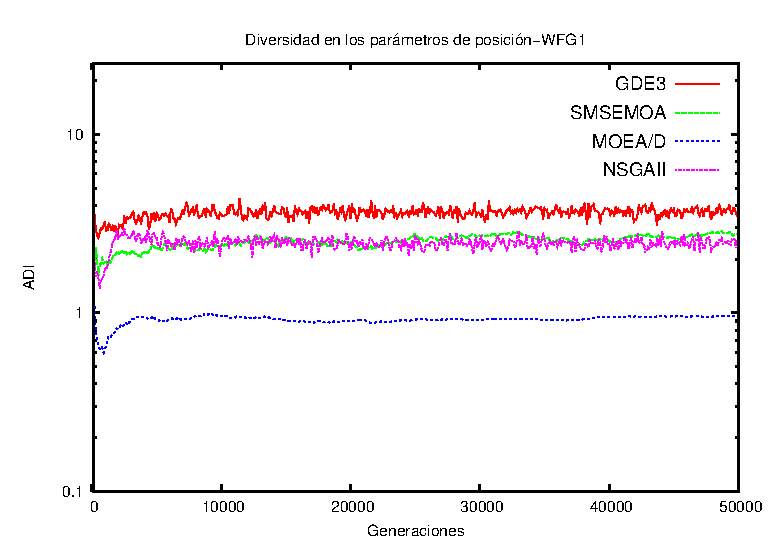
\includegraphics[width=0.5\textwidth]{Figures_Chapter1/Average_PositionParamsStateArt.eps}  
\end{tabular}
\caption{Evolución ADI del estado-del-arte en la instancia WFG1 (escala logarítmica).}
%\caption{Evolution of the DCN for state of art considered (WFG1 instance) in logarithmic scale.}
\label{fig:Average_StateArtDiversityDistanceParameters}
\end{figure}

\begin{figure}[H]
\centering
    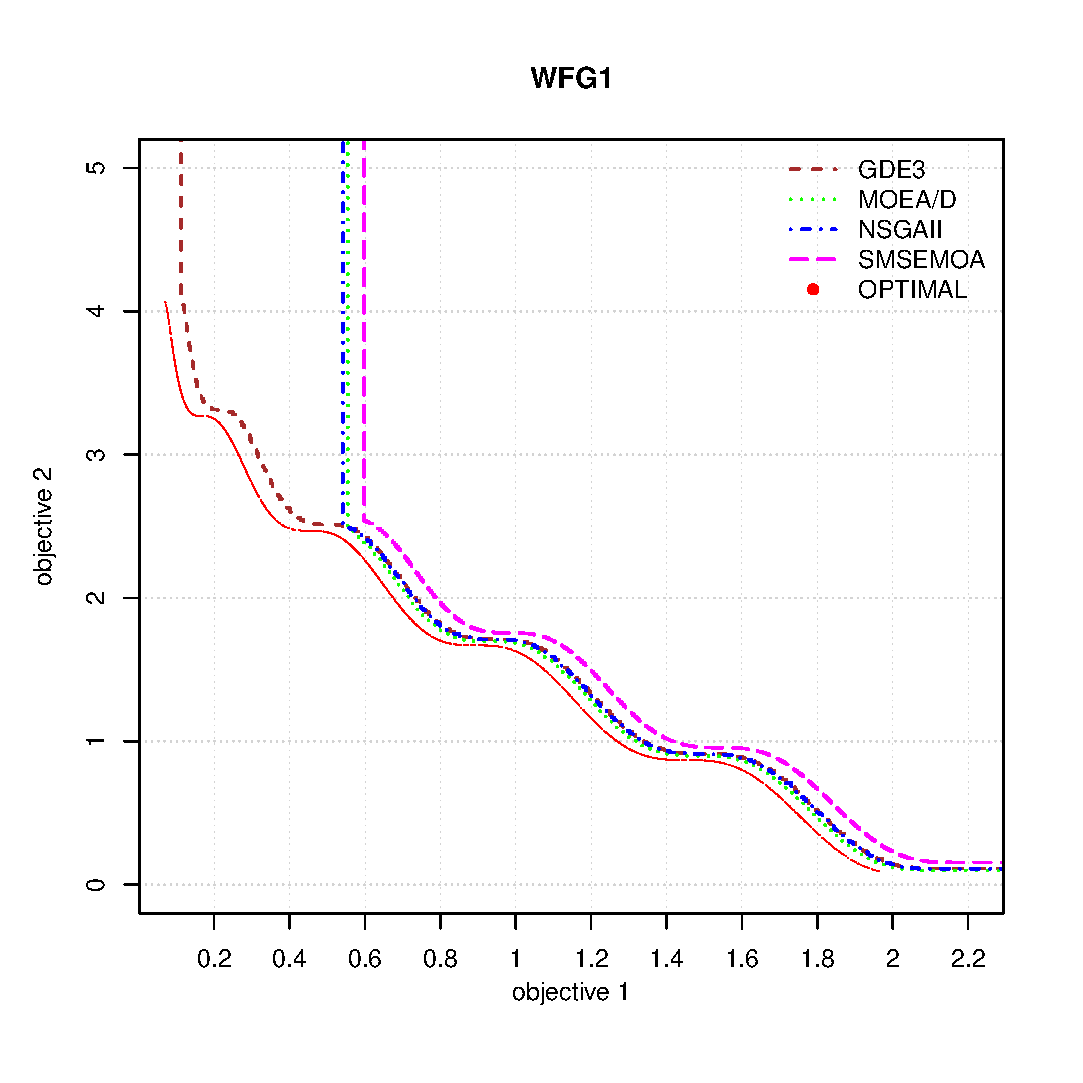
\includegraphics[width=0.5\textwidth]{Figures_Chapter1/WFG1.eps}  
\caption{Superficies de curbimiento logradas al 50\% en el problema de pruena WFG1.}
\label{fig:Superficie_WFG1}
\end{figure}




%In fact, after about 5,000 generations most of the current approaches have completely lost the diversity in the distance parameters subset. Thus, when taking into account this subspace, it can be considered that all these approaches converge prematurely, meaning that in long-term executions, most of the generations are wasted by these algorithms. 
%In this paper we prove that considering diversity in variable space can offer better approximations of the Pareto fronts and that some difficulties related to premature convergence can be avoided. In order to properly prove these facts, the hyper-volume metric and adequate statistical tests are reported. Additionally, attainment surfaces are taken into account. Some of the most difficult problems such as the WFG8 are readily solved by our proposal. However, some difficulties appear in the WFG6 and WFG9. The reasons of these drawbacks are related to the fact that the mating restrictions considered in this paper, provokes a bias to create more individuals in the regions placed near the corners of the search space. Thus, when some of these regions have some promising, but non-optimal solutions, convergence to such regions might appear.



\section{Organización de la tesis}

El presente documento consta de siete capítulos donde se describe el trabajo realizado, los resultados obtenidos y las conclusiones.
%
A continuación, se explica de forma breve el contenido de los siguientes capítulos.
%

En el \textbf{Capítulo \ref{Chapter2}}, se definen formalmente los conceptos en el ámbito multi-objetivo, se presenta una recopilación de los MOEAs más importantes en la literatura.
%
Además se describen los algoritmos utilizados como el estado-del-arte, donde es elegido al menos uno de cada categoría de los MOEAs: basado en dominancia, basado en descomposición y basado en indicadores.
%
También se hace una recopilación de los problemas de referencia ampliamente utilizados (ZDT, DTLZ, WFG y UF).
%
Al final de este capítulo se describen algunas de las técnicas para medir el desempeño de las soluciones generadas por un MOEA.
%

El \textbf{Capítulo \ref{Chapter3}} presenta una revisión de los MOEAs que consideran la diversidad en el espacio de la variables como parte del proceso de búsqueda.
%
Específicamente, es propuesto el VSD-MOEA siendo el primer algoritmo de su tipo, ya que considera la diversidad en el espacio objetivo y en el espacio de las variables simultáneamente, además es basado en dominancia.
%

En el \textbf{Capítulo \ref{Chapter4}} se realiza una revisión de la literatura sobre algunas estrategias para mejorar el mecanismo de emparejamiento y/o remplazo, de igual forma se revisan algunos de los métodos generadores de pesos y se presenta detalladamente el método generador que es implementado en este trabajo.
%
Posteriormente, se presentan tres propuestas algorítmicas basadas en descomposición, el primero mantiene la diversidad de las variables de forma implícita y los otros dos de forma explícita.
%

En el \textbf{Capítulo \ref{Chapter5}} es presentado un análisis del operador genético de Cruce Binario Simulado (SBX) y de los operadores de evolución diferencial en esquemas de diversidad a largo plazo.

La validación experimental es llevada a cabo en el capítulo \textbf{Capítulo \ref{Chapter6}}, donde se realizan pruebas estadísticas, se muestran superficies de cubrimiento logradas y se hacen un análisis de escalabilidad en las variables con la propuesta inicial de dominancia.


%
Finalmente, en el \textbf{Capítulo \ref{Chapter7}} se presentan las conclusiones en base a los resultados obtenidos en este documento, además se discuten los trabajos futuros a desarrollar como resultado de esta investigación.
